\documentclass[12pt,a4paper,notitlepage]{report}

\usepackage[polish, english]{babel}
\usepackage[T1]{fontenc}
\usepackage[utf8]{inputenc}
\usepackage[top=2.5cm, bottom=2.5cm, left=3.5cm, right=2.5cm]{geometry}
\usepackage{indentfirst}
\usepackage{float}
\usepackage{array,multirow,graphicx}
\usepackage{subcaption}
\usepackage{wrapfig}
\usepackage{cite}
\usepackage{gensymb}
\usepackage{arydshln}
%\usepackage{courier}

\setlength{\dashlinedash}{0.5pt}


\makeatletter

\renewcommand{\maketitle}{\begin{titlepage}

    \begin{center}
    \LARGE Uniwersytet Przyrodniczy we Wroc\l{}awiu\\
    \Large Wydzia\l{} Biologii i Hodowli Zwierz\k{a}t\\
    \large Kierunek: Bioinformatyka\\
    Studia stacjonarne drugiego stopnia\\
    Specjalno\'s\'c: Biostatystyka i programowanie bioinformatyczne
    \end{center}

    \vspace{3cm}

    \begin{center}
    \huge \@author \\
    \large 115962
    
    \vspace{2cm}
    
     \textbf{\Huge \@title}
     \end{center}

    \vspace{5cm}
    
    \begin{flushright}
     {\large Praca wykonana pod kierunkiem:}\\
         dr Anna Mucha\\
         Katedra Genetyki
     \end{flushright}

    \vspace*{\stretch{6}}

    \begin{center}
    \Large Wroc\l{}aw, 2020
    \end{center}

  \end{titlepage}%
}

\makeatother

\author{Aneta Sowi\'nska}
\title{Analysis of selected indicators for tonsillectomy}
\linespread{1.3}

\begin{document}

%---------------- Strona tytułowa -----------------

\maketitle


%------------------ Podziękowanie ------------------

\thispagestyle{empty}
\begin{flushright}
  \null\vfill
  \large
  \itshape
  \rightskip=1cm
  Za inspirację, wyrozumiałość oraz pomoc\\
   w trakcie realizacji niniejszej pracy\\
   pragnę złożyć serdecznie podziękowania\\
   mojej promotor, dr Annie Mucha.\\
  \vspace{1cm}
\end{flushright}



%------------------- Abstrakt -------------------

\clearpage
\linespread{1.3}
\begin{abstract}
\vspace{0.5cm}
\begin{center}
\textbf{Analysis of selected indicators for tonsillectomy}
\end{center}
\vspace{0.5cm}

The role of palatine tonsils and the eligibility criteria for tonsillectomy have been widely discussed for many years. Despite being a part of the immune system, in particular pathological states tonsils cease to fulfill their defensive function and become an infection focus.
Both improper recurrent tonsillitis treatment and tonsillectomy carry a risk of dangerous complications. 
Therefore, determining the correct criteria for this kind of surgery is crucial.

The aim of the study was to investigate the connections between chronic tonsillitis and halitosis as an indicator for tonsillectomy. 
Bootstrapping was used since it has considerable advantages when applied to small size data or to non-normal data. 
Most of available literature is more concerned with the mathematical aspects of bootstrap,  however, the use of this technique in medicine and other fields, including biological sciences, is becoming more common.
Also, a Principal Component Analysis is gaining popularity among scientists analyzing medical data.

Analysis of the available data showed that both techniques produced more satisfying results when compared to conventional statistical methods. 
Halitosis in patients with chronic tonsillitis requires numerous additional laboratory tests and the exclusion of all other possible causes like dental and microbiological examination. After exclusion of these, halitosis might be considered as an independent indication for tonsillectomy. \\ \\

\textbf{Keywords:} bootstrap, halitosis, Principal Component Analysis, statistical inference, tonsillectomy.

\end{abstract}

\addcontentsline{toc}{section}{Abstract}

%------------------ Spis treści -------------------

\tableofcontents


%-----------Pocztek części zasadniczej-----------

\clearpage
\linespread{1.3}
%------------------Introduction--------------------
\chapter{Introduction}

The analysis of medical data is characterized by the difficulty of statistical verification of its results, but the health care industry struggles also with issues around data storage and access, data quality, pipeline reliability, privacy and security. With increasing computational power, resampling methods such as bootstraping are becoming more common methodology for investigating problems arising during data-driven model building.

Moreover, these methods can be used in order to overcome problems of datasets with insufficient sizes. This approach helps in building a probability distribution based on much larger number of observations, and thus statistical inference. In general, resampling consists of multiple repetitions of a sample drawing procedure. Based on samples taken from the original data, certain conclusions are drawn about the distribution of a population\cite{Efron93}.

The main purpose of this article is to present one of the possible resampling methods - the bootstrap method - and its application in the analysis of medical data. Also, Principal Component Analysis is considered to be an effective method to reduce the dimensionality of data to a few principal variables that explain most of the variance present in the original data, as well as to characterize the mutual positions of observations under given conditions. A hypothesis for the following analysis assumed that halitosis can be an indication of tonsillectomy.


\section{The structure and role of tonsils}

Tonsils belong to a system of lymph tissue clusters located in the pharynx, on the joint section of respiratory and digestive tracts. The so-called Waldeyer's tonsillar ring was described in 1884 by Wilhelm von Waldeyer, and apart from two palatine tonsils, it also includes pharyngeal tonsil, lingual tonsil and two tubal tonsils \cite{Lapinska16}.

Among them, the palatine tonsils are the biggest and resemble 2 cm long and 1 cm wide ellipsoidal formations. Their structure and location causes that they contribute to the immunological barrier for the reaching food and respiratory antigens.

Within the tonsil, there are numerous clusters of lymphoid tissue (lymphoid follicles). Within a few days after stimulation with the bacterial antigen, more B and T lymphocytes are produced, which disappear after about 3 weeks after cessation of contact with the antigen. Among immunoglobulins, IgG (to 65\%) and IgA (30\%) are the most numerous \cite{Niedzielska03}. 

Hence, tonsils' main function is to inform the system about the presence of food and respiratory antigens, as well as to participate in their destruction by initiating local and general defense reactions.


\section{Indications of tonsillectomy}

As a result of chronic or recurrent inflammatory processes sick tonsils cease to fulfill a defensive function and often contribute to development of autoimmune diseases. Therefore, their role has been discussed for many years. There can be many reasons for dangerous complications, and the very common of these is improper (recurrent) tonsillitis treatment \cite{Niedzielska03}.

Sometimes the only appropriate therapeutic option for diseased palatine tonsils is their surgical removal, so-called tonsillectomy. This treatment has a very long history, since it has already been performed in ancient India and Rome. Present method involving the removal of whole palatine tonsils with various modifications, was first presented by George Waugh in 1909 \cite{McNeill60}.

A better understanding of the role of tonsils in the functioning of the immune system resulted in greater caution in deciding on tonsillectomy. However, the indicators for surgery are still the subject of numerous discussions among specialists.

Before qualifying for tonsillectomy, the frequency of acute bacterial tonsillitis is determined. For children, 7 or more episodes in the last year, 5 or more episodes  per year in the last 2 years, or 3 and more episodes per year in the last 3 years, are indications for tonsillectomy. One episode consists of a sore throat and at least one of the following symptoms: temperature greater than 38.3\degree C, tonsillar exudate, cervical adenopathy, or positive test for group A b-hemolytic streptococcus \cite{Baugh11}.

In adult patients, tonsillectomy is fewer performed as in children. Chronic (recurrent) tonsillar infections recurring several times a year rather than tonsillar hypertrophy are more frequently a reason. Two groups of indications appear to be recognized here: absolute and relative\cite{Niedzielska03,WongChung18}. The first includes: 
\begin{itemize}
	\item tonsil hypertrophy causing apnea during sleep or during wakefulness, 
	\item recurrent hemorrhagic tonsillitis, 
	\item suspected malignant tonsil tumor,
	\item other.
\end{itemize}
The second group includes: 
\begin{itemize}
	\item recurrent/chronic tonsillitis, 
	\item dysphagia, 
	\item inflammation of the lymph nodes associated with a chronic inflammation of the tonsils, 
	\item general complications of chronic tonsillitis, 
	\item hypertrophy of tonsils, 
	\item bleeding from the tonsil.
\end{itemize}


\section{Halitosis as a symptom of chronic tonsillitis}

Chronic tonsillitis most often develops as a result of absence or incorrect treatment of angina \cite{Bochnia05}. Food debris, exfoliated epithelial cells and bacteria remaining in the expanded crypts might form repentant plugs over time. As a consequence of a prolonged inflammatory process, ulceration or fibrosis of the tonsil tissue might occur. These conditions favor the development of aerobic and anaerobic bacteria, as well as fungi. Chronic tonsillitis is one of the reasons for palatine tonsils removal.

Halitosis, defined as a bad breath, is often a symptom of chronic tonsillitis. However, it can be caused by many other factors too. The unpleasant odor might be related to cavities, periodontal disease, poor oral hygiene or other dental problems. Also, respiratory diseases, gastrointestinal diseases, hepatic, pancreatic and nephritic insufficiencies might be the source of a problem. In addition, certain foods or drinks sometimes result in temporary malodorous.

The presence of various substances in the exhaled air is directly responsible for unpleasant odors. These substances arise as products of bacterial   metabolism and are formed by the decomposition of organic material, such as food debris, exfoliated epithelial cells, dead leukocytes, and others. The degradation of proteins, peptides and amino acids containing thiol groups leads to the formation of compounds such as indols, skatols, volatile sulfur compounds (VSC) including hydrogen sulfide, methyl mercaptan and dimethyl sulfide responsible for the odor.

Studies have shown that halitosis reflects complex interactions between several oral Gram-negative bacteria, most of which are anaerobes, however no particular bacterial strain is responsible for the condition \cite{Kotti15}.


%------------Material and methods --------------
\chapter{Material and methods}
\section{Material}

41 patients including 29 women and 13 men, ranging age from 18 to 56 years (mean 27.02, SD 7.86) with chronic tonsillitis and halitosis were qualified for tonsillectomy and therefore selected for the study. A detailed anamnesis was conducted by otolaryngologists and dentists, and microbiological tests were carried out in the laboratory of the Academic Clinical Hospital in Wroclaw. Also, routine laboratory tests and two surveys were conducted in order to eliminate causes of halitosis other than those indicative of tonsillitis. Patients answered questions related to their medical history, food habits, smoking cigarettes and oral hygiene. 
Those who confirmed the occurrence of any gastrointestinal, pulmonary or other systemic metabolic disorders in the survey were eliminated from the research group.
Another exclusion criteria included smokers, heavy alcoholic drinkers, improper oral hygiene and \textit{Helicobacter pylori} carriers. Dental examination excluded also patients with carious lesions, exposed tooth pulps, peridonthal diseases and thick tongue coat.

\section{Methods}

Patients underwent both subjective and objective evaluation of oral odor. 
For \mbox{a subjective} assessment of an unpleasant odor in the mouth each patient underwent organoleptic examination before tonsillectomy. Patients were neither allowed to take antibiotics for a period of three weeks, consume garlic, onion and spicy dishes for 24 hours nor apply perfume. Within 12 hours, it was also recommended to avoid food intake and drinks, brush teeth, use breath fresheners and smoke cigarettes. During the study, the smell of air exhaled through the mouth was compared with the smell of air exhaled through the nose (when mouth closed). The patient then exhaled into a transparent tube 10 cm long and 2.5 mm in diameter. In order to assess the intensity of the unpleasant smell from the mouth a six-grade Rosenberg scale was used which is the most widely used scale of halitosis \cite{Rosenberg92}. The odor was classified between 0 and 5, where: 0 - absence of odor, 1 - barely noticeable odor, 2 - slight malodor, 3 - moderate malodor, 4 - strong malodor and 5 - severe malodor.\

For objective assessment of halitosis each patient underwent a Man-hal-II Halimeter test. This sulfide monitor measures volatile sulfur compounds such as hydrogen sulfide, methyl mercaptan and dimethyl sulfide which are contributing factors for halitosis. Each sample was taken after 3 minute re-stabilization period when patients were breathing through the nose with  mouths kept closed. During the test the device's straw was inserted into the subject’s mouth and one was asked to exhale briefly for 30 seconds. 
The procedure was repeated in three trials for each patient and the peaks' values were recorded in parts per billion (ppb) sulfide equivalents \cite{Alasqah16}.
In order to obtain reliable results, patients could not eat, drink, smoke, chew gum, brush their teeth, use the brush, fresheners or oral hygiene products for 12 hours prior to the halimetric test. It was also recommended not to use cosmetics such as perfumes, aftershave or lipstick. \

Organoleptic and halimetric examination was repeated for each patient, at least 2-3 months after removal of the palatine tonsils and completion of the healing process.

The average value of the three VSC measurements was used for further statistical analysis. Depending on the chosen criterion of division, two or three groups of patients have been distinguished. First one considered 100 ppb as threshold dividing group into normal (when below) and abnormal (when above the threshold). Second, more detailed criterion included intermediate states as follows: the range up to 100 ppb considered as correct, 100 - 180 ppb as a light form of disease and above 250 ppb as a severe one \cite{Lee04}. However, the study group did not include patients belonging to the latter (Fig. \ref{fig:Fig_2.1}).  

\begin{figure}[hbt!]
	\centering
	\begin{subfigure}[b]{0.85\textwidth}
		\centering
		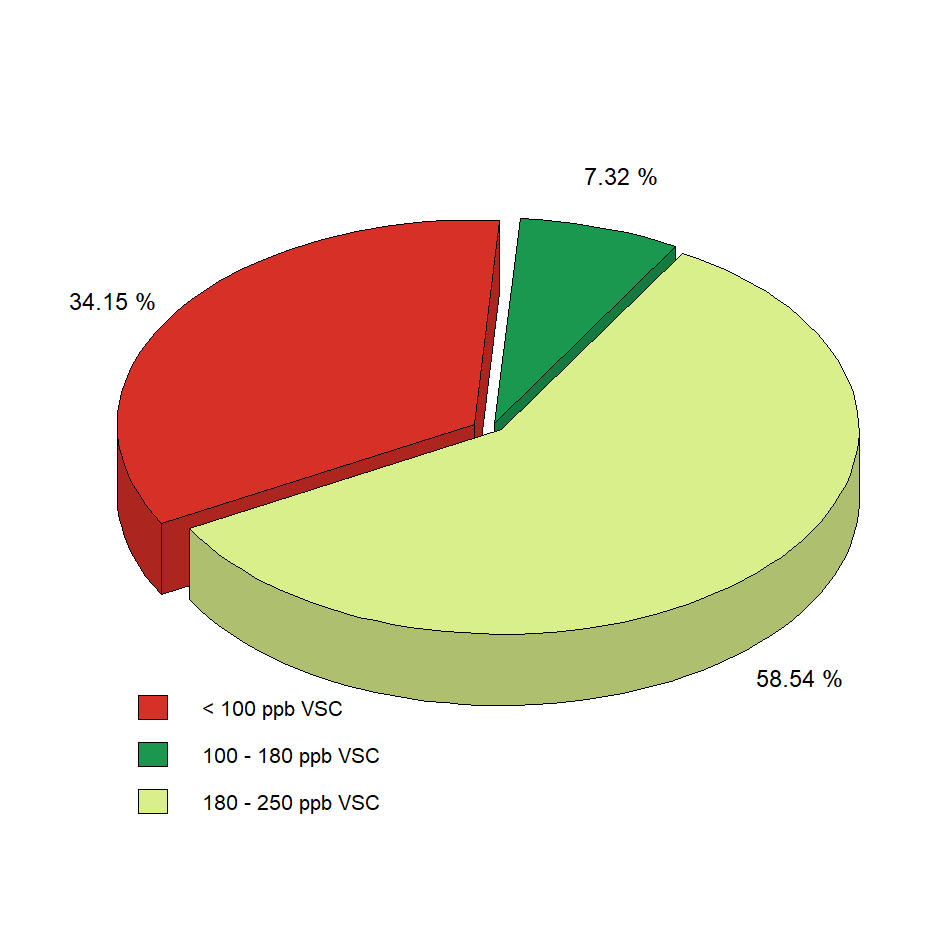
\includegraphics[width=.8\textwidth, height=.7\textwidth]{./Figures/Fig_2.1a2} 
		\caption{the ratio of groups with different forms of the disease}
		\label{fig:Fig_2.1a}
	\end{subfigure} 
	\vspace*{2cm}
	
	\begin{subfigure}[b]{0.85\textwidth}
		\centering
		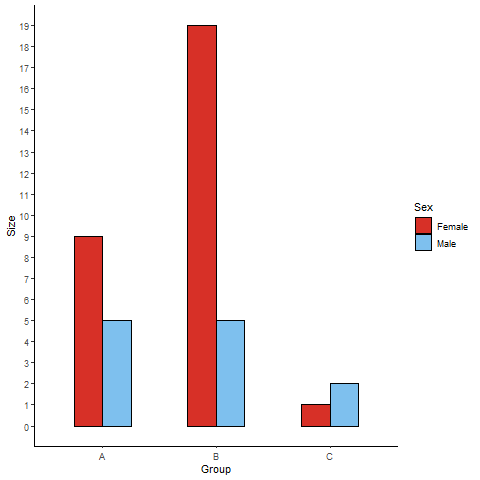
\includegraphics[width=0.9\textwidth, height=.7\textwidth]{./Figures/Fig_2.1b2}
		\caption{the gender distribution within groups A: < 100 ppb,  B: 100 - 180 ppb, C: > 180 ppb VSC}
		\label{fig:Fig_2.1b}
	\end{subfigure}
	 
	\caption{Groups of patients due to the level of VSC before tonsillectomy.}
	\label{fig:Fig_2.1}
\end{figure}

%---PCA---
A Principal Component Analysis (PCA) was used in order to validate the classification above. This method enables finding the directions of maximum variance in high-dimensional data and project it onto a smaller dimensional subspace while retaining most of the information. In the following work, a self-written R script \mbox{(R version 3.6.3)} was used to conduct the overall analysis. R is a programming language and free software environment used for statistical computing and visualizations supported by the R Foundation for Statistical Computing \cite{RCoreTeam13}. PCA was performed using \texttt{FactoMineR} which is an R package dedicated to multivariate Exploratory Data Analysis \cite{factominer08}, as well as \texttt{factoextra} to extract and visualize the results \cite{factoextra13}. There are also other, built-in R functions avaliable - \texttt{princomp()} and \texttt{prcomp()} from  \texttt{stats} package \cite{RCoreTeam13}. The preceding one uses the spectral decomposition approach, while the functions \texttt{prcomp()} and \texttt{FactoMineR::PCA()} use the singular value decomposition.

Comparisons between groups and within groups were made using appropriate statistical tests from the \texttt{stats} package as described in the third chapter. The \texttt{stats} package is part of R and contains functions for statistical calculations and random number generation \cite{RCoreTeam13}. All tests were preceded by checking the assumptions authorizing to carry them out. The gender distribution was included in each comparison. 
The significance level $\alpha$ for the tested models was 5\% ($\alpha$ = 0,05).

%---Bootstrap---
The bootstrap was performed by a self-written R code. Each bootstrap sample was drawn 1000 times. Beside distribution parameters for continuous data, standard errors, biases and confidence intervals were calculated. Appropriate tests were performed on bootstrap populations and compared with the outcomes of statistical inference conducted on the original sample.

%---Other packages---
In addition, the following packages were used:
\begin{itemize}
\item \texttt{tidyverse}, \texttt{dplyr} for data manipulation \cite{tidyverse19, dplyr18},
\item \texttt{moments}  to calculate skewness in data \cite{moments15},
\item \texttt{plotrix}, \texttt{ggplot2}, \texttt{corrplot} for data visualization \cite{plotrix06, ggplot216, corrplot17}.
\end{itemize}



%--------------------- Results ---------------------
\chapter{Results}

The first stage of the analysis involved examining the population of forty-one patients qualified for the study. The respondents were divided into four groups on the basis of a halitometry cut-off value: Group A - normal (below 100 ppb), Group B - minor halitosis (100 - 180 ppb), Group C - abnormal halitometry (180 - 250 ppb) and Group D - severe or chronic form of halitosis (above 250 ppb).  None of the patients showed symptoms, classifying him or her to the latter, therefore Group D was not presented in the results. 

The first section summarizes the distribution of age, living place, education, profession and halitometry results for the observed data. 

The second section presents the results of Principal Component Analysis examining the adequacy of the assignment of patients to groups.

Due to the relatively small research sample's size, the statistical inference procedure was repeated in conjunction with bootstrap technique. The results were posted at the end of this chapter.

%---Original data statistical inference---
\section{Original sample results}

%---General statistics---
Table \ref{tab:General_stats} summarizes the comparison of features: age, living place, profession and education between men and women in the original data. Student's \mbox{t test} (\texttt{stats::t.test}) was used to test the significance of differences in means of age after checking normality of the distribution and homogeneity of variance. Those assumptions were verified each time with Shapiro-Wilk Normality Test (\texttt{stats:: shapiro.test}) and F Test to Compare Two Variances (\texttt{stats::var.test}). 
Categorical data - living place, profession, education - were tested with Fisher's Exact Test for Count Data (\texttt{stats::fisher.test}) since the condition for  $\chi^2 $ test of independence (number of observations in a single cell greater than 5) was not fulfilled. 
No statistically significant difference was observed in terms of analyzed features (p > 0.05). 

\begin{table}[H]
\centering
	\begin{tabular}{lcccc}
	\hline 		 				& \textbf{Female} & \textbf{Male} & \textbf{Total} &  \textbf{Comparison} \\
	 		 					& n = 29 		& n = 12		& n = 41		&  (\textit{p-value}) \\
	\hline
	\hline
	\bf{Age}						&			&			&			&		\\
	\indent mean					& 26.69		& 27.83		& 27.02		& 		\\
	\indent sd					& 8.49		& 6.32		& 7.86		& 0.6391 \\
	\indent me					& 24.00		& 27.00		& 25.00		& 		\\
	\indent range				& 18.00-56.00 & 19.00-36.00	& 18.00-56.00	& \\
	\hline
	
	\bf{Living place} 				&			&			&			&		\\
	\indent village				& 5 (17.24)	& 0 (0.00)	& 5	(12.20)	& 		\\
	\indent town					& 2 (6.90)	& 1	(8.33) 	& 3	(17.85) 	&  0.3078 \\
	\indent city					& 22 (75.86)	& 11 (91.67) & 33 (80.49) & 		\\
	\hline
	
	\bf{Profession} 				&			&			&			&		\\
	\indent school-age student		& 2 (6.90)	& 2 (16.67)	& 4	(9.76) 	& 		\\
	\indent student				& 6 (20.69)	& 1	(8.33) 	& 7	(17.10) 	& 0.1834 \\
	\indent blue-collar worker		& 3 (10.35)	& 4 (33.33) 	& 7 (17.10) 	& 		\\
	\indent white-collar worker	& 18 (62.07)	& 5 (41.67) 	& 23 (56.10)	 & 		\\
	\hline
	
	\bf{Education} 				&			&			&			&		\\
	\indent elementary			& 1 (3.45)	& 2 (16.70)	& 3	(7.32) 	& 		\\
	\indent secondary			& 13 (44.80)	& 5	(41.70) 	& 18 (43.90) 	& 0.2699 \\
	\indent higher				& 15 (51.70)	& 5 (41.70) 	& 20 (48.80) 	& 		\\
	\hline
	
	\end{tabular} \\ 
	\caption{General statistics for studied sample and comparisons between female and male.}
	\label{tab:General_stats}
\end{table}





%---Halitometry---
The comparisons of VSC levels between men and women were made with Wilcoxon test (\texttt{stats::wilcox.test}) due to heterogeneity of variance between groups. According to p-values 0.5378 and 0.8185, the null hypothesis saying that the mean VSC levels for women and men were equal both before and after tonsillectomy failed to reject (Tab. \ref{tab:Halitometry_results}). 

Levels of VSC before and after tonsillectomy (for whole sample) were compared using a paired Student's t test (\texttt{stats::t.test}) after bringing the prior to a normal distribution. Originally, the average level of VSC had a right-skewed distribution with coefficient  = 0.787. Taking a square root of this variable turned out to be enought to decrease the coefficient of skewness to 0.018 which is close to zero and meet the assumptions of normality in Shapiro-Wilk Normality test \cite{Wilcox18}.
According to p-value < 0.05, the null hypothesis about equality of the average VSC levels in both groups was rejected, thus the distributions of those variables differed significantly. The level of VSC in the exhaled air was effectively lowered as a result of tonsillectomy.

\begin{table}[H]
\centering
	\begin{tabular}{lcccc}
	\hline 					& \textbf{Female} & \textbf{Male}	& \textbf{Total} 	&  \textbf{Comparison}  \\
	 				 		& n = 29 			& n = 12		& n = 41			&  (\textit{p-value}) \\
	\hline
	\hline
	\bf{Before}				&				&			&				&		\\
	\indent mean				& 115.03			& 107.92		& 113.00			& 		\\
	\indent sd					& 37.89			& 67.81		& 47.76			& 0.5378 \\
	\indent me				& 120.00			& 105.00		& 117.00			& 		\\
	\indent range				& 22.00-186.00 	& 25.00-238.00	 & 22.00-238.00	& 		\\
	\hline
	
	\bf{After}					&				&			&				&		\\
	\indent mean				& 43.52			& 45.08		& 43.98			& 		\\
	\indent sd					& 19.20			& 24.81		& 20.66			& 0.8185 \\
	\indent me				& 50.00			& 36.00		& 40.00 			& 		\\
	\indent range				& 7.00-80.00	 	& 23.00-113.00	& 7.00-113.00		& 		\\
	\hline
	
	\end{tabular} \\ 
	\caption{Halitometry results: levels of VSC before and after tonsillectomy.}
	\label{tab:Halitometry_results}
\end{table}

There was only one patient left with minor halitosis after the removal of palatine tonsils - a 29-year old man with 113 ppb of VSC.
In general, the avarage level of VSC dropped by 106.50 ppb compared to pre-tonsillectomy measurements as shown in the Figure \ref{fig:Fig_3.1}.


\begin{figure}[H]
	\centering
	\begin{subfigure}[b]{0.85\textwidth}
		\centering
		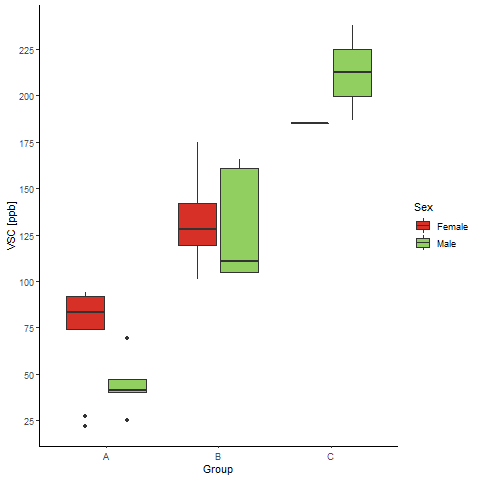
\includegraphics[width=.9\textwidth, height=.75\textwidth]{./Figures/Fig_3.1a2} 
		\caption{before tonsillectomy}
		\label{fig:Fig_3.1a}
	\end{subfigure} 
	\vspace*{2cm}
	
	\begin{subfigure}[b]{0.85\textwidth}
		\centering
		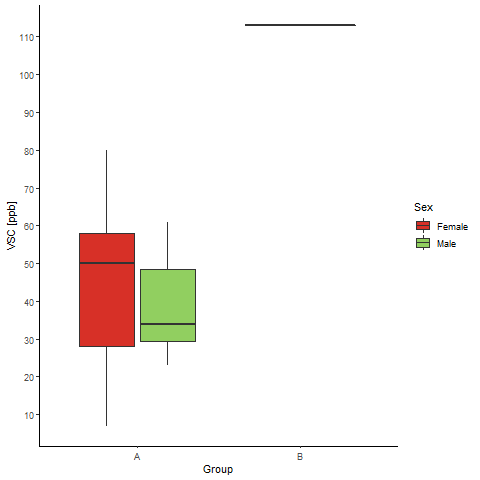
\includegraphics[width=.9\textwidth, height=.75\textwidth]{./Figures/Fig_3.1b2}
		\caption{after tonsillectomy}
		\label{fig:Fig_3.1b}
	\end{subfigure}
	 
	\caption{Levels of VSC in groups with split on gender. Group A: < 100 ppb, Group B: 100 - 180 ppb, Group C: > 180 ppb VSC.}
	\label{fig:Fig_3.1}
\end{figure}



%---PCA---
\newpage
\section{PCA results}

Since Principal Component Analysis can be applied only to numerical problems, a subset of numerical variables from the original data was created. The analysis concerned the following features: age, three VSC measurements before and VSC three measurements after tonsillectomy, two averages of these measurements, height and weight (41 individuals and 11 variables in total). This subset of data was used as an input to \texttt{FactoMineR::PCA} function which created an object containing information listed below: 

\begin{enumerate}
\item \texttt{\$eig} - eigenvalues
\item \texttt{\$var} - results for the variables
\item \texttt{\$var\$coord} - coordinates for the variables
\item \texttt{\$var\$cor} - correlations variables - dimensions
\item \texttt{\$var\$cos2} - cos2 for the variables
\item \texttt{\$var\$contrib} - contributions of the variables
\item \texttt{\$ind} - results for the individuals
\item \texttt{\$ind\$coord} - coordinates for the individuals
\item \texttt{\$ind\$cos2} - cos2 for the individuals
\item \texttt{\$ind\$contrib} - contributions of the individuals
\item \texttt{\$call} - summary statistics
\item \texttt{\$call\$centre} - mean of the variables
\item \texttt{\$call\$ecart.type} - standard error of the variables
\item \texttt{\$call\$row.w} - weights for the individuals
\item \texttt{\$call\$col.w} - weights for the variables.
\end{enumerate}

An important stage preceding the proper analysis of data is their standarization in order to avoid falsifying the obtained results. This is particularly recommended when variables are measured in different scales (e.g ppb, kilograms, centimeters) but also when the mean or the standard deviation of variables are largely different. After scaling the obtained variables are comparable and have standard deviation one and mean zero. The function \texttt{PCA()} standardizes the data by default.

In order to determine the minimum number of principal components (PCs) that account for most of the variation in analyzed data two methods were used. The first one was based on the proportion of variance that the components explain. The acceptance level of variance was set to 80\%, thus PC3 might be taken as the cut-off point (Tab. \ref{tab:Eigenvalues}).

\begin{table}[H]
\centering
	\begin{tabular}{lrrr}
	\hline \textbf{PC}  & \textbf{eigenvalue}	& \textbf{pct of variance} & \textbf{cumulative pct of variance}  \\
	\hline
	\hline
	comp 1		&	5.3278		&	48.434			&	48.4342\\
	comp 2		&	2.0581		&	18.7102			&	67.1444\\
	comp 3		&	1.7014		&	15.4671			&	82.6115\\
	\hdashline
	comp 4		&	0.9906		&	9.0054			&	91.6170\\
	comp 5		&	0.3051		&	2.7735			&	94.3905\\
	comp 6		&	0.2083		&	1.8938			&	96.2843\\
	comp 7		&	0.1968		&	1.7896			&	98.0738\\
	comp 8		&	0.0944		&	0.8585			&	98.9323\\
	comp 9		&	0.0705		&	0.6406			&	99.5729\\
	comp 10		&	0.0467		&	0.4245			&	99.9974\\
	comp 11		&	0.0003		&	0.0026			&	100.0000\\
	\hline
	\end{tabular} \\ 
	\caption{The eigenvalues and percentages of explained variance for corresponding principal components.}
	\label{tab:Eigenvalues}
\end{table}

An alternative method of estimating the number of principal components is a scree plot (Fig. \ref{fig:Fig_3.2}), which sorts the eigenvalues in descending order. The number of PCs is selected at the point where there is \mbox{a relative} decrease in the amount of variance explained by given component. In that case, both methods indicated the same cut-off point which was the third principal component (PC3) meaning that first three principal components explain 82.61\% of variation in the data.

\begin{figure}[hbt!]
	\centering
	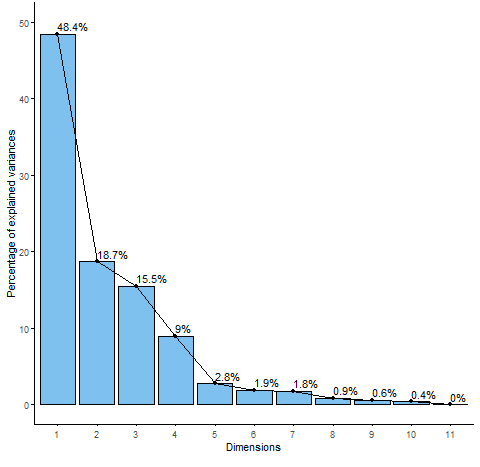
\includegraphics[width=0.87\textwidth]{./Figures/Fig_3.2}
	\caption{Scree plot.}
	\label{fig:Fig_3.2}
\end{figure}	

Examining magnitude and direction of coefficients for the original variables allowed to interpret each principal component. In these results, first and second principal component had positive associations with the average levels of VSC (before and after tonsillectomy), so this component primarily measured surgery effectiveness. The second component had positive associations with individual levels of VSC, so this component primarily measured repeatability of results. The third component had large positive associations with height and weight, so this component primarily measured the patient's body mass index (\ref{tab:Var_coordinates}). 

\begin{table}[H]
\centering
	\begin{tabular}{lrrr}
	\hline \textbf{Variable}  & \textbf{Dim.1}	& \textbf{Dim.2} & \textbf{Dim.3}\\
	\hline
	\hline
	Age				&	0.06474271 	 	&	0.2142688  	&	3.8189970\\
	Meas. Ia			&	12.98299405  	&	9.8236148  	&	0.4125337\\
	Meas. Ib			&	11.68182094  	&	14.8535097  	&	1.3612200\\
	Meas. Ic			&	13.19998598  	&	8.0359692  	&	1.0841263\\
	Avg Meas. Ia-c	&	13.94205852  	&	11.5795143  	&	1.0594427\\
	Meas. IIa		&	11.75608497  	&	12.2961987  	&	0.8804465\\
	Meas. IIb		&	11.57708848  	&	13.7652005  	&	0.6844923\\
	Meas. IIc		&	11.00329721  	&	13.4237281  	&	0.2559425\\
	Avg Meas. IIa-c	&	13.45587482  	&	9.8219842  	&	0.9707230\\
	Height			&	0.04792823  		&	2.3886855  	&	45.0820763\\
	Weight			&	0.28812409  		&	3.7973262  	&	44.3899997\\
	\hline
	\end{tabular} \\ 
	\caption{Contribution of variables is first three principal components.}
	\label{tab:Var_coordinates}
\end{table}

\newpage
A PCA biplot visualizes both principal component scores of the observations (so called \textit{score plot}) and loadings of variables (a \textit{loading plot}). In general, a biplot is a projection of high-dimensional space onto a two-dimensional plane. In the Figure \ref{fig:Fig_3.3} all different-shaped points are the projected observations and vectors are the projected variables. Each observation is displayed in the figure keeping its original axes \cite{Zhang17}. 

Biplots permit a broad interpretation. For instance, points situated closely to each other represent intuitively the observations with similar values. In the figure below clusters were identified on the basis of pre-tonsillectomy VSC levels and 95\% confidence ellipses were added. The centroids mark the barycentres of the points belonging to the same cluster.

\begin{figure}[H]
	\centering
	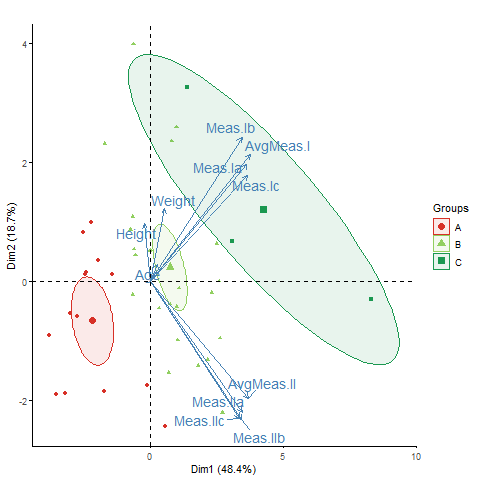
\includegraphics[width=\textwidth, height=.91\textwidth]{./Figures/Fig_3.3.3}
	\caption{A biplot showing both principal component scores for individuals categorized into three groups and loadings of variables}
	\label{fig:Fig_3.3}
\end{figure}	


The relative coordinates of an observation might be approximated by projecting the point onto the variable vectors. However, since the vectors have been centered and scaled they cannot be used to estimate the exact coordinates.

Next, the cosine of the angle between pairs of vectors represents a correlation between the corresponding variables. Highly correlated variables point in similar directions, while uncorrelated variables are nearly perpendicular to each other. As can be noticed, all variables associated with VSC measurements before tonsillectomy (Meas.Ia, Meas.Ib, Meas.Ic and AvgMeas.I) were closely correlated. The same applied to VSC measurements after tonsillectomy (Meas.IIa, Meas.IIb, Meas.IIc and AvgMeas.II). At the same time, pre- and post-surgery VSC levels did not correlate with each other indicating significant differences and the effectiveness of tonsillectomy.
 
Finally, the cosine of the angle between a vector and an axis suggests the importance of contribution of the corresponding variable to the principal component. It would appear that Height and Weight have the biggest impact on the second principal component. However, looking at Table \ref{tab:Var_coordinates} with exact contributions of variables it is clear that those variables had the biggest impact on PC3 instead of PC2. 
    
Age did not seem to have a notable impact on understanding relationships in the data.


%--- Bootstrap ---
\section{Bootstrap results}
Based on the drawn bootstrap samples, the distributions parameters of features describing the studied group were estimated. A few algorithms to specify the number of replicates in the bootstrap procedure might be found in the literature. According to Efron and Tibshirani  B = 500 is usually sufficient for the general standard bootstrap method \cite{Efron93}. However, the computation of confidence intervals or tests of significance require a larger number of bootstrap replicates. Thus, this parameter was set to 1000 in the current study \cite{Pattengale10, Davison97}.

Table \ref{tab:General_stats_boot} summarizes the results of the bootstrap procedure. 
A variety of sample statistics, such as the mean, standard deviation, median and range was calculated for women, men and whole bootstrap population.
The $\chi^2 $ goodness of fit test (\texttt{stats::chisq.test}) was performed for the categorical data in opposite to Fisher's Exact Test for Count Data which was performed for the original sample.
The variable of Age was compared with the Wilcoxon test due to the lack of normal distribution.

At 0.05 significance level, the null hypothesis saying that the patients (either within one sex or between both sexes) are equally distributed across education, profession and living place, was rejected. Also, the null hypothesis saying that the age of female and male come from identical distribution was not accepted.


\begin{table}[H]
\centering
	\begin{tabular}{lcccc}
	\hline 		 			& \textbf{Female} & \textbf{Male} 	& \textbf{Total} &  \textbf{Comparison} \\
	 		 				& B = 1000 		& B = 1000	& B = 1000	&  (\textit{p-value}) \\
	\hline
	\hline
	\bf{Age}					&			&			&				&		\\
	\indent mean				& 26.68		& 27.87		& 27.02			& 		\\
	\indent sd				& 8.11		& 6.00		& 7.63			& < 0.05 * \\
	\indent me				& 24.44		& 27.83		& 25.09			& 		\\
	\indent range			& 18.39-51.86 	& 19.42-35.56	& 18.35-51.87 		&	 	\\
	\hline
	
	\bf{Living place} 			&				&				&				&		\\
	\indent village			& 161 (16.10)	& 0 (0.00)		& 113 (11.30)	& 		\\
	\indent town				& 68 (6.80)		& 90 (9.00) 		& 79 (7.90) 		&  < 0.05 *\\
	\indent city				& 771 (77.10)	& 910 (91.00) 	& 808 (80.80) 	& 		\\
	\hline
	
	\bf{Profession} 			&			&			&				&		\\
	\indent school-age student	& 61 (6.10)	& 166 (16.60)	& 92 (9.20) 		& 		\\
	\indent student				& 194 (19.40)	& 104 (10.40) 	& 181 (18.10) 		& < 0.05 *\\
	\indent blue-collar worker		& 110 (11.00)	& 313 (31.30) 	& 147 (14.70) 		& 		\\
	\indent white-collar worker	& 635 (63.50)	& 417 (41.70) 	& 580 (58.00) 		& 		\\
	\hline
	
	\bf{Education} 				&			&			&				&		\\
	\indent elementary			& 27 (2.70)	& 171 (17.10)	& 72 (7.20) 		& 		\\
	\indent secondary			& 432 (43.20)	& 417 (41.70) 	& 444 (44.40) 		& < 0.05 *\\
	\indent higher				& 541 (54.10)	& 412 (41.20) 	& 484 (48.40) 		& 		\\
	\hline
	
	\end{tabular} \\ 
	\caption{General statistics for bootstrap population.}
	\label{tab:General_stats_boot}
\end{table}


Subsequently, the distribution parameters were estimated for the average VSC measurements taken both before and after the tonsillectomy. All samples differed in terms of distribution; therefore Wilcoxon test  was used for comparisons of halitometric effects in both sexes (Tab. \ref{tab:Halitometry_results_boot}). In opposite to the original sample comparison outcome, a significant difference was observed between women and men before tonsillectomy, and p-value for the test after tonsillectomy was close to the significance level $\alpha$ = 0.05.


\begin{table}
\centering
	\begin{tabular}{lcccc}
	\hline 				& \textbf{Female} & \textbf{Male} 	& \textbf{Total} 	&  \textbf{Comparison}  \\
	 				 	& B = 1000 		& B = 1000 		& B = 1000 		&  (\textit{p-value}) \\
	\hline
	\hline
	\bf{Before}			&			&			&			&		\\
	\indent mean			& 114.71		& 108.01		& 113.06		& 		\\
	\indent sd				& 36.89		& 64.08		& 46.68		& 4.340e-13 *\\
	\indent me			& 118.86		& 100.19		& 115.40		& 		\\
	\indent range			& 30.02-179.59 & 30.74-217.15 & 24.17-217.99&		 \\ 
	\hline
	
	\bf{After}				&			&			&			&		\\
	\indent mean			& 43.40		& 45.17		& 43.69		&		\\
	\indent sd				& 18.82		& 22.67		& 20.07		& 0.052	\\
	\indent me			& 45.21		& 38.35		& 42.07		&		\\
	\indent range			& 9.93-75.27	& 24.15-95.53	& 9.96-98.21	&		\\ 
	\hline
	\end{tabular}
	\caption{Halitometry results for bootstrap population: levels of VSC before and after tonsillectomy.}
	\label{tab:Halitometry_results_boot}
\end{table}

In order to evaluate the model, accuracies of the estimates were calculated. The results for estimated mean values were presented in Table \ref{tab:Estimates_accuracy}. The 95\% confidence intervals were assessed calculating the 2.5 and 97.5 percentiles of the differences in bootstrapped means. The obtained biases were insignificant what indicated very small differences between means calculated for original and bootstrap samples.

Not surprisingly, the standard error for VSC level before tonsillectomy in the group of male was the highest one. Also, in the original sample the dispersion of this measure was large (Fig. \ref{fig:Fig_3.1a}). Generally, the estimated distribution parameters were satisfying.

\begin{table}[H]
\centering
	\begin{tabular}{lcccc}
	\hline 		 		& \textbf{Mean} 	& \textbf{Standard error} & \textbf{Bias} &  \textbf{Confidence intervals} \\
	\hline
	\hline
	\bf{Female}				&			&			&				&					\\
	\indent Age				& 26.68		& 1.490		& 0.004			& (23.965; 29.759)		\\
	\indent VSC before			& 114.71		& 7.320		& 0.333			& (98.894; 128.693)		\\
	\indent VSC after			& 43.40		& 3.428		& 0.113			& (36.584; 50.277)		\\
	\hline
	
	\bf{Male} 					&			&			&				&					\\
	\indent Age				& 27.87		& 1.777		& 0.402			& (24.417; 31.417)		\\
	\indent VSC before			& 108.01		& 18.930		& 0.096			& (73.147; 145.096)		\\
	\indent VSC after			& 45.17		& 6.804		& 0.092			& (33.417; 59.417)		\\
	\hline
	
	\bf{Total} 				&			&			&				&					\\
	\indent Age				& 27.02		& 1.185		& 0.003			& (24.877; 29.538)		\\
	\indent VSC before			& 113.06		& 7.462		& 0.113			& (98.830; 128.722)		\\
	\indent VSC after			& 43.69		& 3.136		& 0.288			& (37.790; 49.881)		\\
	\hline
	\end{tabular} 
	\caption{The accuracy of the mean estimates for age and halitometry results.}
	\label{tab:Estimates_accuracy}
\end{table}

The concentration of VSC after removal of palatine tonsils decreased on average by 68.976 ppb, falling within confidence intervals (-84.591; -52.434).
The demonstrated decrease of 61\% was statistically significant (p < 0.05) due to Wilcoxon signed rank test with continuity correction outcome. 

The difference in VSC between two bootstrap populations was clearly performed in histograms below. With more resamples, Figure \ref{fig:Fig_3.4}  showed that the shape of obtained bootstrap distribution appeared to be normal. Although the bootstrap sample should have a similar center and spread as the original sample, there were some significant differences that might result from small sample sizes.

\begin{figure}[H]
	\centering
	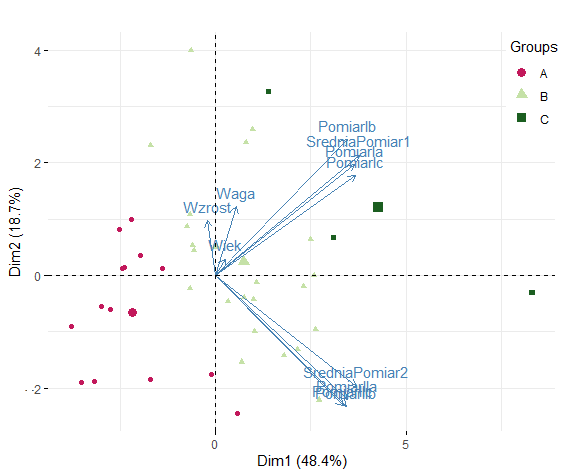
\includegraphics[width=.9\textwidth, height=.85\textwidth]{./Figures/Fig_3.4}
	\caption{Histograms of VSC levels in the original samples and bootstrap populations.}
	\label{fig:Fig_3.4}
\end{figure}	


%--------------- Discussion ----------------
\chapter{Discussion}

%Halitosis affects about 25–30\% of world’s population. Tonsillectomy is one of the most frequently performed surgeries in the world in the practice of laryngologists \cite{Blustoniec77}. About 400,000 are performed annually in the US these treatments. 

Discussions on the role of the tonsils and the qualifying criteria for tonsillectomy last for many years. 
Despite being a part of immune system that defends against infections, tonsils cease to fulfill a defensive function and become an infection focus as a result of chronic inflammatory processes.

Dangerous complications might occur in consequence of improper (recurrent) tonsillitis treatment, as well as after tonsils removal. The decision to perform tonsillectomy must be made in a responsible and thoughtful manner. Therefore, determining the correct criteria for this surgery is crucial.

The aim of the study was to investigate connections between chronic tonsillitis and halitosis as tonsillectomy indicator. 
Due to many other possible indications for removal of palatine tonsils, a restrictive selection of patients was necessary and the final sample size was equal 41.

Halitosis was assessed using two common methods - organoleptic and halitometric. A positive correlation was observed between Rosenberg's score and VSC concentration both before and after surgery. Higher Pearson coefficients was obtained while comparing VSC levels measured before tonsillectomy in comparison to the outcomes of measurements after the surgery. The effectiveness of the organoleptic method seems to depend on VSC level which makes it less effective (Fig. {\ref{fig:RSES_correlation}}). The more intense the problems with the unpleasant odor, the better the coverage of organoleptic and halimetric test results. Although the organoleptic evalutaion with six-level scale seems to give better results when compare to three-level scale \cite{MesquitaGuimaraes17}, both compared methods should be used complementarily, not separately.

\begin{figure}[h]
	\centering
	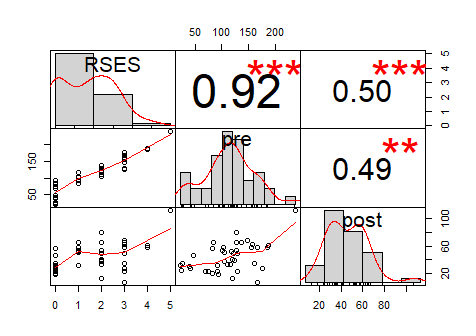
\includegraphics[width=0.7\columnwidth]{./Figures/RSES_correlation}
	\caption{Correlation between Rosenberg scores and halitometry outcomes. RSES - Rosenberg scale, pre - VSC level before tonsillectomy, post - VSC level after tonsillectomy.}
	\label{fig:RSES_correlation}
\end{figure}	

General statistics provided on the studied sample showed that there was no difference between men and women in context of age, living place, profession or education. A small negative correlation was demonstarted between VSC level and living place (-0.28 before and -0.34 after tonsillectomy). However, the size of the group and unequal proportion of men and women (29 \textit{vs} 12) did not make these results reliable. Therefore, a bootstrap technique was performed.

The bootstrap method enabled to obtain satisfactory results in the analysis of medical data. The applied resampling procedure gave the possibility of statistical inference without making any assumptions on the examined features' distributions. Furthermore, it allowed to obtain empirical distributions of very large numbers although research sample was not big. It is essential especially in case of statistical inference based on medical data, because confirming the effectiveness of therapy or inferring the frequency of a rare disease entity can only rely on big amount of good quality data.

Increasing the size of compared bootstrap populations to 1000 showed that there was a significant difference between men and women in context of age, living place, profession or education. 

In both bootstrap and classical statistical inference, the level of VSC in the exhaled air was effectively lowered as a result of tonsillectomy. This seems to confirm that halitosis can be effectively eliminated by tonsillectomy. Unfortunately, we do not have enough information to conclude that the surgery was effective regarding to chronic tonsillitis. For this purpose, the study should be repeated after an appropriate period of time after surgery.

In 2014 Burton et al. compared the clinical effectiveness and safety of both tonsillectomy and adenotonsillectomy (removal of the tonsils and adenoid tissues) against non-surgical treatment with chronic tonsillitis. Authors concluded that the operation reduced the number of episodes of sore throat and days with sore throat in children in the first year after surgery. However, the overall impact of surgery was summed up as modest. While insufficient information was available on the effectiveness in adults, more severely affected children were more likely to benefit because of a small reduction in moderate or severe sore throat episodes \cite{Burton14}.

In context of bootstrap, Davison and Kuonen \cite{Davison03} stressed that considering this method as an alternative for classical statistics is misguided. The authors warn before using such a powerful tools as resampling technics without deep understanding why it works. They emphasized the importance of monitoring the output in order to ensure that the results make sense and understand how the output will be used. Therefore, bootstrap should always be preceded by population, samples parameters, and fundamental statistical notions examinations. The following work considers these observations.

In order to reduce the number of dimensions of data as well as to check the relevance of thresholds dividing into groups of observations (A, B and C), a Principal Component Analysis was performed. PCA analysis reports as many PCs as the number of variables included in the analyses. However, we can observe that the first three PCs are responsible for the majority of the variance in the data which is 82.61\%. 
The group allocation also seems to be consistent, as can be seen from the biplot (Fig. \ref{fig:Fig_3.3}) in which group B is the most numerous and group C is the least numerous.

Results of PCA for other data sets are often more challenging. More predictors included in the PCA might result in a bigger number of PCs selected, and thus increase the model size. In general, it aims to select the principal components with the largest variance in order to keep only those explaining enough variance to make epidemiological and clinical sense \cite{Zhang17}.

To sum up, described techniques might complement  nonparametric statistical methods and should, where appropriate, be included in data processing methodologies. The methods have proved to be useful especially in the analysis of medical data.


%--------------- Bibliografia ---------------

\begin{thebibliography}{26}
\bibliographystyle{plain}

\bibitem{Efron93} Efron B, Tibshirani RJ (1993) \emph{An Introduction to the Bootstrap}, Chapman \&  Hall. 

\bibitem{Lapinska16} Łapińska I, Zawadzka-Glos L (2016) \emph{Adenoid and tonsils hypertrophy - Symptoms and treatment}, New Medicine 20(4): 103-106.

\bibitem{Niedzielska03} Niedzielska G. (2003) \emph{Postępowanie w nawracających zapaleniach migdałków podniebiennych u dzieci}, Otorynolaryngologia 2(1): 8–10.

\bibitem{McNeill60} McNeill RA (1960) \emph{A History of Tonsillectomy: Two Millenia of Trauma, Haemorrhage and Controversy}, Ulster Medical Journal 29(1): 59-63. 

\bibitem{Baugh11} Baugh RF et al. (2011) \emph {Clinical practice guideline: tonsillectomy in children},  Otolaryngology-Head and Neck Surgery, 144: S1-S30.

\bibitem{WongChung18} Wong Chung JERE et al. (2018) \emph{Tonsillotomy Versus Tonsillectomy in Adults Suffering From Tonsil-Related Afflictions: A Systematic Review}, Acta Otolaryngologica 138(5): 492-501.

%\bibitem{Burton08} Burton M. Commentary (2008) \emph{Tonsillectomy — then and now},  International Journal of Epidemiology 37, 23–25.

\bibitem{Bochnia05} Bochnia M, Dziewiszek W, Rostkowska-Nadolska (2005) \emph{Tonsylektomia w XXI wieku}, Family Medicine \& Primary Care Review 7:  874–881.

\bibitem{Kotti15} Kotti AB, Subramanyam RV (2015) \emph{Oral malodor: A review of etiology and pathogenesis}, Journal of Dr. NTR University of Health Sciences 4(1): 1-7.

\bibitem{Rosenberg92} Rosenberg M, McCulloch CAG (1992) \emph{Measurement of Oral Malodor: Current Methods and Future Prospects}, Journal of Periodontology 63: 776–782.

\bibitem{Alasqah16} Alasqah M, Khan S, Elqomsan MA, Gufran K, Kola Z, Bin Hamza MO (2016) \emph{Assessment of halitosis using the organoleptic method and volatile sulfur compounds monitoring}, Journal of Dental Research and Review 3(3): 94-98.

\bibitem{Lee04} Lee PP, Mak WY, Newsome P (2004) \emph{The aetiology and treatment of oral halitosis: an update}, Hong Kong Medical Journal  10: 414–418.

\bibitem{RCoreTeam13} R Core Team (2013) \emph{R: A language and environment for statistical computing}, R Foundation for Statistical Computing, Vienna, Austria. URL http://www.R-project.org/.

\bibitem{factominer08} L\^e S, Josse J, Husson F (2008) \emph{FactoMineR: A Package for Multivariate Analysis}, R package version 2.3. Journal of Statistical Software 25(1): 1–18.

\bibitem{factoextra13} Kassambara A, Mundt F (2013) \emph{factoextra: Extract and Visualize the Results of Multivariate Data Analyses}, R package version 1.0.6.

\bibitem{tidyverse19} Wickham H et al. (2019) \emph{Welcome to the tidyverse}, Journal of Open Source Software 4(43): 1686.

\bibitem{dplyr18} Wickham H et al. (2018) \emph{dplyr: A Grammar of Data Manipulation}, R package version 0.8.4. https://CRAN.R-project.org/package=dplyr.

\bibitem{moments15} Komsta L, Novomestky F (2015) \emph{moments: Moments, cumulants, skewness, kurtosis and related tests},  R package version 0.14. https://CRAN.R-project.org/package=moments.

\bibitem{plotrix06} Lemon J (2006) \emph{Plotrix: a package in the red light district of R}, R-News 6(4): 8-12. 

\bibitem{ggplot216} Wickham H (2016) \emph{ggplot2: Elegant Graphics for Data Analysis}, Springer-Verlag New York. ISBN 978-3-319-24277-4, https://ggplot2.tidyverse.org. 

\bibitem{corrplot17} Wei T, Simko V (2017) \emph{R package ,,corrplot": Visualization of a Correlation Matrix}, R package version 0.84.

\bibitem{Wilcox18} Wilcox R, Peterson TJ, McNitt-Gray JL (2018) \emph{Data Analyses When Sample Sizes Are Small: Modern Advances for Dealing With Outliers, Skewed Distributions, and Heteroscedasticity}, Journal of Applied Biomechanics 34(4): 258-261.

\bibitem{Pattengale10} Pattengale ND, Alipour M, Bininda-Emonds OR, Moret BM, Stamatakis A. (2010) \emph{How many bootstrap replicates are necessary?}, Journal of Computational Biology 17(3): 337‐354.

\bibitem{Davison97} Davison AC, Hinkley DV (1997) \emph{Bootstrap Methods and Their Application}, Cambridge, UK: Cambridge University Press.

%\bibitem{Blustoniec77} Blustoniec C (1997) \emph{Status of tonsillectomy and adenoidectomy}, Laryngoscope, 8, 1233.


\bibitem{MesquitaGuimaraes17} de Mesquita‑Guimaraes, et al. (2017) \emph{Organoleptic reproducibility for halitosis}, European Journal of General Dentistry 6(1): 9-13.

\bibitem{Burton14} Burton MJ, Glasziou PP, Chong L, Venekamp RP (2014) \emph{Tonsillectomy or adenotonsillectomy versus non‐surgical treatment for chronic/recurrent acute tonsillitis}, Cochrane Database of Systematic Reviews 11, Art. No.: CD001802.  

\bibitem{Davison03}  Davison AC, Kuonen D (2003) \emph{An Introduction to the Bootstrap with Applications in R}, Statistical Computing \& Statistical Graphics Newsletter 13(1): 6-11.

\bibitem{Zhang17} Zhang Z, Castello A (2017)\emph{Principal components analysis in clinical studies}, Annals of Translational Medicine 5(17): 351.
%Bridge P. D., and Sawilowsky, S. S. (1999), "Increasing Physicians' Awareness of the Impact of Statistics on Research Outcomes: Comparative Power of the t Test and Wilcoxon Rank-Sum Test in Small Samples Applied Research," Journal of Clinical Epidemiology, 52, 229-235
% Skovlund, E.,  andFenstad, G. U. (2001), "Should We Always Choose a Nonpara metric Test When Comparing Two Apparently Nonnormal Distributions?" Journal of Clinical Epidemiology, 54, 86-92. 
%Welch, B.  L. (1938), "The Significance of  the Difference Between Two Means When the Population Variances are Unequal," Biometrika, 29, 350-362. 
%Zimmerman, D. W., and Zumbo, B., D. (1993), "Rank Transformations and the Power of the Student ?-Test and Welch t-Test for Nonnormal Populations with Unequal Variances," Canadian Journal of Experimental Psychology, 47, 523-539. 

\end{thebibliography}

\listoffigures
\addcontentsline{toc}{section}{List of Figures}

\listoftables
\addcontentsline{toc}{section}{List of Tables}

\end{document}